%!TEX root = ../thesis.tex
%*******************************************************************************
%*********************************** Sixth Chapter *****************************
%*******************************************************************************

\chapter{Gluon Propagator on Vortex-Modified Backgrounds}\label{chapter:GluonPropagatorResults}
\ifpdf
    \graphicspath{{Chapter6/Figs/Raster/}{Chapter6/Figs/PDF/}{Chapter6/Figs/}}
\else
    \graphicspath{{Chapter6/Figs/Vector/}{Chapter6/Figs/}}
\fi
\textit{This chapter is based on the paper ``Gluon propagator on a centre-vortex background'', }\citet{Biddle:2018dtc}.

\section{Preliminary Results}
Here we present the results from the gluon propagator, calculated according to method outlined in Chapter~\ref{chapter:GluonPropagator}, on our three vortex-modified configurations.
%
\begin{figure}[tb]
\centering
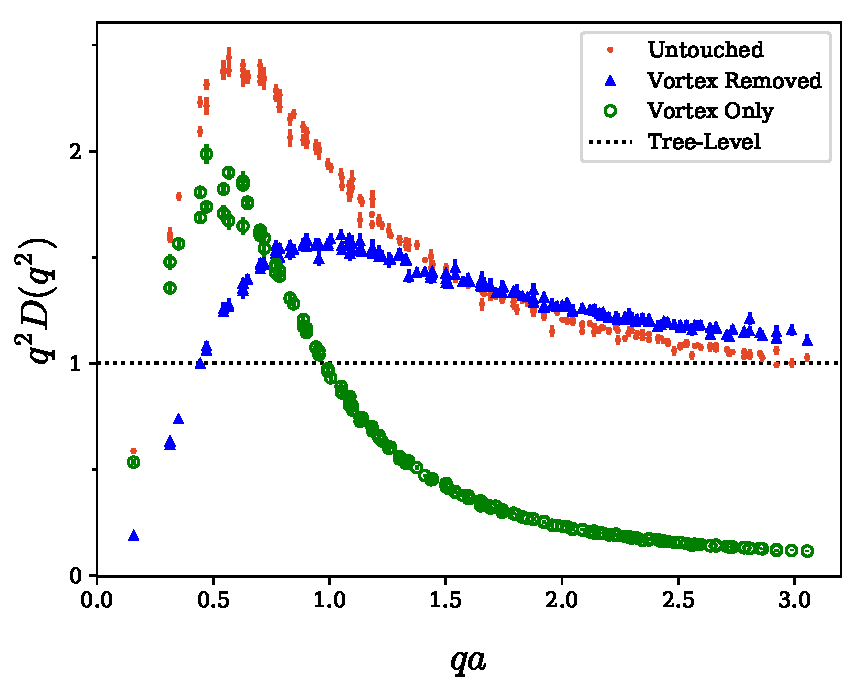
\includegraphics[width=\linewidth]{./ScalarGluComp_q2_NoCoolSum.pdf}
\caption[The gluon propagator calculated from the original untouched, shown with the vortex removed and vortex only results.]{\label{fig:NoCool}The gluon propagator calculated from the original untouched (red dots), shown with the vortex removed (blue triangles) and vortex only (green open circles) results. Here, the renormalisation factor for the vortex removed and vortex only propagators is chosen to be the same as for the untouched propagator.}
\end{figure}
%
\begin{figure}[tb]
\centering
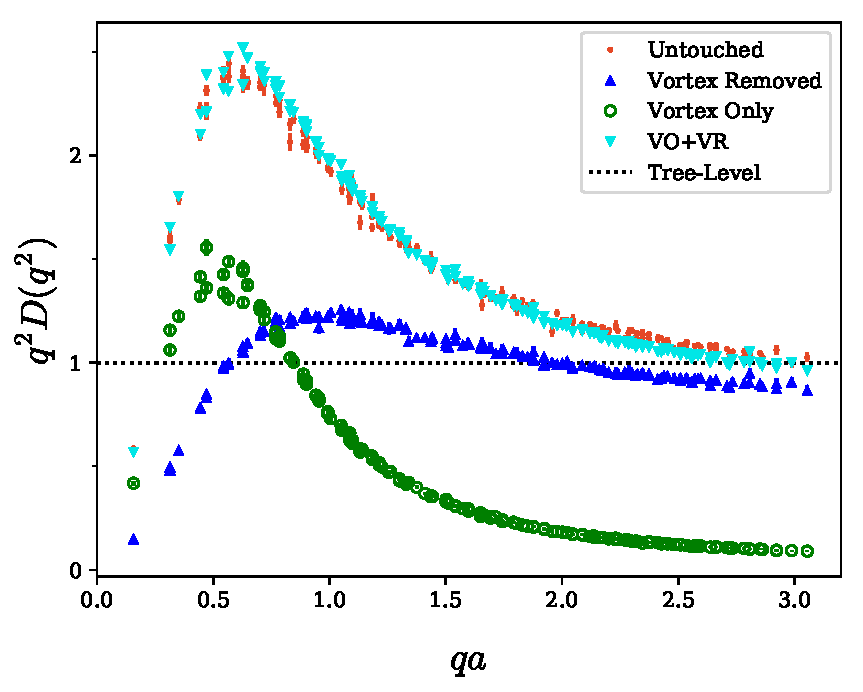
\includegraphics[width=\linewidth]{./ScalarGluComp_q2_NoCoolSum2.pdf}
\caption[The gluon propagator from the original untouched alongside the independently renormalised sum of the vortex removed and vortex only propagators.]{\label{fig:NoCoolSum}The gluon propagator from the original untouched ensemble as in Fig.~\ref{fig:NoCool}, plotted alongside the independently renormalised sum (cyan triangles) of the vortex removed and vortex only propagators. The two vortex modified propagators are also shown, but here their renormalisation factor is chosen to be the same as for the summed propagator.}
\end{figure}
%
Calculating the scalar propagator on untouched, vortex-removed and vortex only configurations gives the results illustrated in Fig.~\ref{fig:NoCool}. To make contact with the tree-level propagator at large $q^2$, we renormalise such that $q^2D(q^2)=1$ for $qa = 3.0$ on the original configurations, and apply this same renormalisation factor to the vortex removed and vortex only propagators. The vortex removed configurations display the expected behaviour, with vortex removal corresponding to significant infrared suppression of the propagator when compared to the untouched propagator, in agreement with the results of Ref.~\cite{Bowman:2010zr}. The increased roughness of the gauge fields after vortex removal is evidenced by the enhancement of the propagator at large $q$. This reflects the increase in short-distance fluctuations that have been introduced to the gauge fields by the vortex removal procedure.\\

It is interesting to note that the vortex only propagator retains approximately two thirds of the untouched propagator's peak strength. This is comparable to previous work showing partial recovery of the string tension on vortex only configurations~\cite{Trewartha:2015ida,Trewartha:2017ive,Langfeld:2003ev,Stack:2002sy}. Despite only recovering a portion of the original strength, the infrared peak is still considerably greater than the peak observed in the vortex removed propagator. The loss of strength is most likely in part because of the known imperfections in the vortex identification algorithm (see Sec.~\ref{sec:LocatingVortices}) that results in some vortex matter remaining in the vortex removed configurations. The vortex only configurations also exhibit a loss of short range strength, due to the absence of the high frequency modes that are instead contained within the vortex removed field.\\

If we sum the vortex only and vortex removed propagators and independently renormalise such that $q^2\,D(q^2)=1$ at $qa=3.0$ (discussed further in Sec.~\ref{sec:Renormalisation}), we obtain the result shown in Fig.~\ref{fig:NoCoolSum}. Here we observe agreement between the untouched and summed propagators. This indicates that vortex modification effectively partitions the lattice configuration into short range physics on the vortex removed configurations and long range physics on the vortex only configurations, up to errors in the vortex identification procedure.

\subsection{Partitioning}

Partitioning of the untouched gluon propagator into vortex removed and vortex only contributions is expected if the vortex only and vortex removed configurations are orthogonal. To see how this behaviour emerges, suppose that we can decompose the gluon field $A_\mu$ into two independent fields as follows
\begin{equation}
  A_\mu(p) = B_\mu(p) + C_\mu(p).
\end{equation}
In the context of this work, we associate $B_\mu$ with the background field of short-range gluon fluctuations and $C_\mu$ with the centre vortex field.
Note also that if $B$ and $C$ are in Landau gauge then so is $A.$ Using this partitioning it follows that the gluon propagator for $A$ can be written as the sum of the respective gluon propagators for $B$ and $C,$
\begin{align}
  D^{A}_{\mu\nu}(p) &= \frac{1}{V}\langle A_\mu(p) \, A_\nu(-p) \rangle\nonumber \\
  &= \frac{1}{V}\Big(\langle B_\mu(p)B_\nu(-p)\rangle + \langle C_\mu(p)C_\nu(-p)\rangle\nonumber\\
   &~~~~~~~+ \langle B_\mu(p)C_\nu(-p)+ C_\mu(p)B_\nu(-p) \rangle\Big)\nonumber \\
  &= D^{B}_{\mu\nu}(p) + D^{C}_{\mu\nu}(p),\label{eq:Partition}
\end{align}
where we have made use of the fact that $B$ and $C$ represent orthogonal degrees of freedom in the gauge field and hence in the ensemble average the cross-correlations should vanish. These cross-correlations are explicitly calculated by evaluating 
\begin{equation}
D_{\text{cross-terms}}(p^2) = \frac { 2 } { 3 \left( n _ { c } ^ { 2 } - 1 \right) V } \left\langle \operatorname { Tr } \left( B_\mu(p)C_\mu(-p)+ C_\mu(p)B_\mu(-p) \right) \right\rangle\, ,
\label{eq:CTprop}
\end{equation}
analogous to the scalar gluon propagator derived in Chapter~\ref{chapter:GluonPropagator}. As can be clearly seen from Fig.~\ref{fig:CrossTerms}, in the ensemble average Eq.~\ref{eq:CTprop} vanishes, indicating that the vortex only and vortex removed configurations truly do represent a orthogonal degrees of freedom.\\ 
%
\begin{figure}[htb!]
\centering
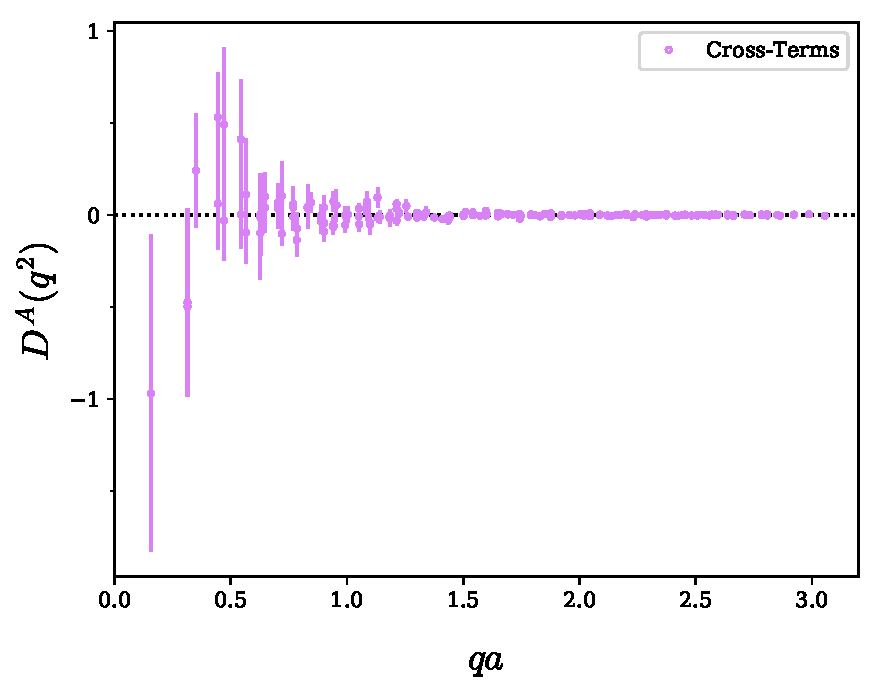
\includegraphics[width=0.9\linewidth]{./ScalarGluComp_q2_CrossTerms.pdf}
\caption{\label{fig:CrossTerms} Calculation of the cross-terms arising from Eq.~\ref{eq:Partition}}
\end{figure} 
%

To elucidate the connection to the unitary formulation of the lattice gauge links, we suppose that we can transform $A$ to an ``ideal centre gauge'' such that in lattice units the field $C$ consists purely of centre phases,
%
\begin{equation}
C_\mu(x) = k\,\frac{2\pi}{3} I,\quad k\in \{-1,0,+1\}.
\end{equation}
%
As $A = B + C$ it immediately follows that we can write
\begin{equation}
U_{\mu}(x) = e^{i B_{\mu}(x+\hat{\mu}/2)} \, e^{i C_{\mu}(x+\hat{\mu}/2)},
\end{equation}
noting that in our ideal centre gauge $[B,C] = 0$ so the Baker-Campbell-Haussdorff relation is trivial. Identifying
\begin{equation}
Z_{\mu}(x) = e^{i C_{\mu}(x+\hat{\mu}/2)}\, ,
\end{equation}
as the vortex-projected field, and
\begin{equation}
R_{\mu}(x) = e^{i B_{\mu}(x+\hat{\mu}/2)}\, ,
\end{equation}
as the background remainder field we thus recover the decomposition of the links used herein,
\begin{equation}
U_{\mu}(x) = Z_{\mu}(x)\cdot R_{\mu}(x).
\end{equation}
In practise, on the lattice the maximal centre gauge fixing that is implemented will differ from the ideal centre gauge postulated here due to apparent numerical difficulties in simultaneously identifying all vortex matter within an $SU(3)$ gauge field. What this means is that the projected field $Z$ may not capture all of the vortex matter such that there is some non-trivial topological structures that remain in the background field $R.$ The infrared enhancement in the vortex removed results in Fig.~\ref{fig:NoCool} suggests this is the case.\\

\subsection{Renormalisation}\label{sec:Renormalisation}

In Fig.~\ref{fig:NoCoolSum} it proved necessary to independently renormalise the untouched and summed propagators such that they agree at $qa=3.0$. The necessity of this renormalisation is worth discussing, as it is important to motivate why comparison between the original and reconstructed propagators is valid. To do this, it is beneficial to first consider the renormalised gluon propagator in the continuum. The renormalised propagator at any loop order, $D_R^\text{C}(q^2)$ can be related to the bare propagator, $D^\text{C}(q^2)$ via the relationship
%
\begin{equation}
D^\text{C}(q^2) = Z^\text{C}_3 \, D_R^\text{C}(q^2)\, .
\label{eq:ContinuumRenormalisation}
\end{equation}
%
Typically $Z^\text{C}_3$ and $D^\text{C}(q)$ are infinite, whereas $D_R^\text{C}(q)$ is finite. The renormalised propagator is not independent of the renormalisation scheme, and the expression for $Z^\text{C}_3$ depends on the renormalisation scheme employed. For example, in the minimal subtraction (MS) scheme at one-loop order with no quark fields, $Z_3^\text{C}=1+\frac{5g^2}{8\pi^2\epsilon}$~\cite{ryder1996quantum}, where the quantity $\epsilon$ is introduced during the analytic continuation to $d = 4-\epsilon$ dimensions as part of the dimensional regularisation procedure. However, regardless of the chosen renormalisation scheme, the renormalised propagator can always be expressed in the form shown in Eq.~\ref{eq:ContinuumRenormalisation}~\cite{vanRitbergen:1997va}.\\

On the lattice, we can explicitly calculate the now finite bare dimensionless propagator $D^\text{L}(q^2)$, as the lattice introduces an explicit momentum cutoff of $\frac{\pi}{a}$. In the language of the continuum, this can be thought of as an approximation of the continuum bare propagator to all loop orders. Similarly, the lattice renormalisation constant $Z_3(\mu, a)$ is also finite. On the lattice, Eq.~\ref{eq:ContinuumRenormalisation} becomes
%
\begin{equation}
a^2 D^\text{L}(q^2) = Z_3(\mu, a)\, D_R(q^2)\, ,
\label{eq:LatticeRenormalisation}
\end{equation}
%
where the $a^2$ factor restores the dimensionality of the left-hand side of the equation. Despite the finiteness of $D^\text{L}(q^2)$ and $Z_3(\mu, a)$, it is still necessary to enforce a renormalisation scheme to be able to draw meaningful comparisons between propagators. As such, we employ the momentum space subtraction (MOM) scheme~\cite{Bowman:2004jm,Leinweber:1998uu,Bonnet:2001uh}, which requires that for some sufficiently large $\mu$
%
\begin{equation}
D_R(q^2)\big|_{q^2=\mu^2}=\frac{1}{\mu^2}\, .
\end{equation}
%
This sets the value of the renormalisation constant to be
%
\begin{equation}
Z_3(\mu,a) = a^2 \, \mu^2 \, D^\text{L}(\mu^2)\, ,
\end{equation}
such that
%
\begin{equation}
D_R(q^2) = \frac{D^\text{L}(q^2)}{\mu^2 \, D^\text{L}(\mu^2)}\, .
\end{equation}
%
This renormalised propagator is what we plot in e.g. Fig.~\ref{fig:NoCoolSum}. The value of $\mu$ is arbitrary, however it is necessary that it is sufficiently large such that it is outside the infrared region where the gluon propagator exhibits substantial deviation from tree-level behaviour. Furthermore, $\mu$ must be away from the momentum cutoff, as the renormalisation constant is only independent of the cutoff in the limit that the cutoff tends towards infinity~\cite{Bonnet:2001uh,Boucaud:2006pc}. Given the momentum range of $qa\in [0,4.6]$, arising from the momentum variables described in Sec.~\ref{sec:MomentumVariables}, a choice of $\mu =3.0$ satisfies both conditions. Additionally, it also falls below the maximum momentum of $qa = 3.06$ imposed by the momentum half-cut described in Sec.~\ref{sec:LatticeParameters}. Once the renormalisation scheme has been imposed, it is then possible to connect the lattice results with those obtained from perturbation theory by connecting the renormalisation constant with those obtained from the MS or modified minimal subtraction (\textoverline{\text{MS}}) schemes.\\

This discussion of renormalisation has motivated why it is acceptable to compare the untouched and summed propagators: it is the renormalised propagator, not the bare propagator, that carries the physical meaning. Hence, the fact that the untouched and summed propagators agree after renormalisation in Fig.~\ref{fig:NoCoolSum} is an important result indicating the effective partitioning of the gluon propagator under vortex modification. The final point to be discussed is the renormalisation applied to the vortex only and vortex removed propagators. Given that we don't have an {\it a priori} expectation of the tree-level behaviour, imposing the MOM condition lacks meaning. Instead, to facilitate comparisons, we make use of the original $Z_3(\mu, a)$ obtained for the untouched propagator unless specified otherwise. Maintaining this consistency is sufficient to comment on the qualitative shape of the propagator, which is the most significant point of interest in this research. 

%\textcolor{red}{\textbf{Renormalisation steps:}
%\begin{enumerate}
%\item Calculation contains divergent integrals that must be isolated.
%\item Dimensional regularisation isolates the infinities in the integral.
%\item Redefine the mass/coupling to absorb these infinities. The new constant is \textit{finite}, whereas the original constant is taken to be \textit{infinite}.
%\item Alternatively, the counter term method can be used.
%\item The counter term method states that the original constant is \textit{finite}, that are modified by infinite constants.
%\item Upon calculating physical quantities, the infinite constants cancel off the infinities arising from the loop integrals.
%\end{enumerate}
%\textbf{Questions:}
%\begin{enumerate}
%\item At what scale does $D_{\text{QED}}(q^2) = \frac{1}{q^2}$?
%\item At what scale can we suppose that $D_{\text{QED}}(q^2) = D_{\text{QCD}}(q^2)$
%\item Is it reasonable to say that the condition that must be enforced on the combined propagator is $D(q^2) = \frac{1}{q^2}$ at some large momentum, and as such this is the normalisation that should be applied to the VR and VO propagators?
%\item Does $D_{\text{QCD}}(q^2)$ equal the bare continuum propagator at a fixed cutoff?
%\item What does the renormalised propagator correspond to in the continuum? 
%\end{enumerate}
%}

\section{Impact of Cooling}
We now perform 10 sweeps of cooling on the untouched, vortex-removed and vortex-only ensembles, the results of which are shown in Fig.~\ref{fig:10SweepsCooling}. As is typical of cooling, the removal of short range structures means that all three ensembles tend to zero as $q\rightarrow\infty$. There is now a noticeable improvement in the agreement between the untouched and vortex only configurations; however there is still a difference present, especially in the $qa\approx0.5$ and $qa\approx1.5$ regions.\\
%
\begin{figure}[htb!]
\centering
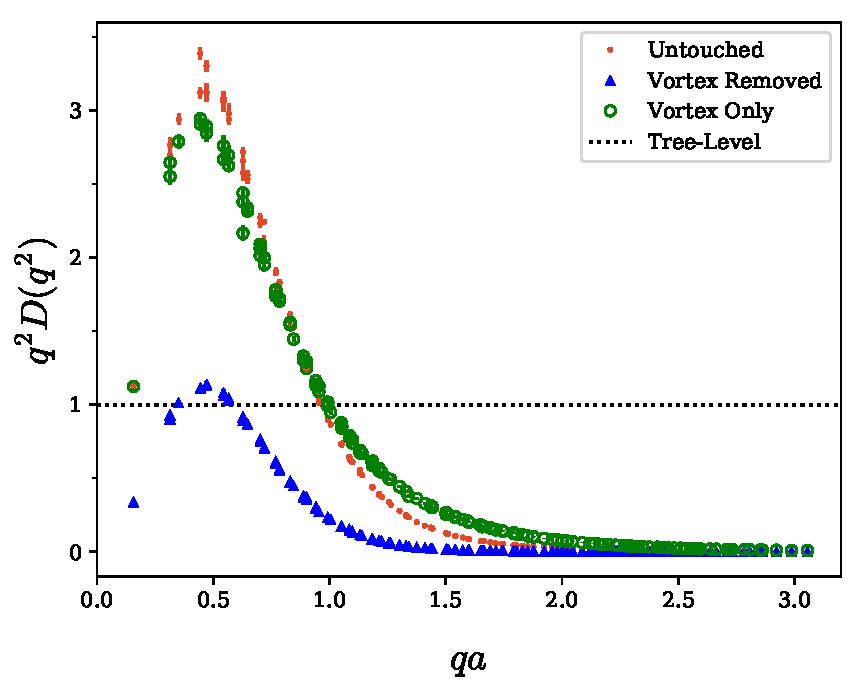
\includegraphics[width=\linewidth]{./ScalarGluComp_q2_10sweepsAll.pdf}
\caption[The gluon propagator calculated on the three ensembles after 10 sweeps of cooling.]{\label{fig:10SweepsCooling}The gluon propagator calculated on the three ensembles after 10 sweeps of cooling. We now observe an improved agreement between the untouched and vortex only propagators.}
\end{figure}  
%

We perform the same analysis of the vortex only propagator under cooling as performed in Sec.~\ref{sec:CoolingGluProp} on the untouched propagator. Once again in gauge fixing, each sweep is preconditioned by the Landau gauge transformation of the previous sweep in descending order. The result of this analysis is shown in Fig.~\ref{fig:1to10VO}. This figure shows a similar change in the vortex only propagator when compared to the untouched propagator in Fig.~\ref{fig:1to10SweepsCooling}, with an enhancement in the infrared and suppression in the UV modes. The UV suppression is less noticeable in this case due to the prior removal of short range effects brought about by the vortex identification.\\

%
\begin{figure}[htb!]
\centering
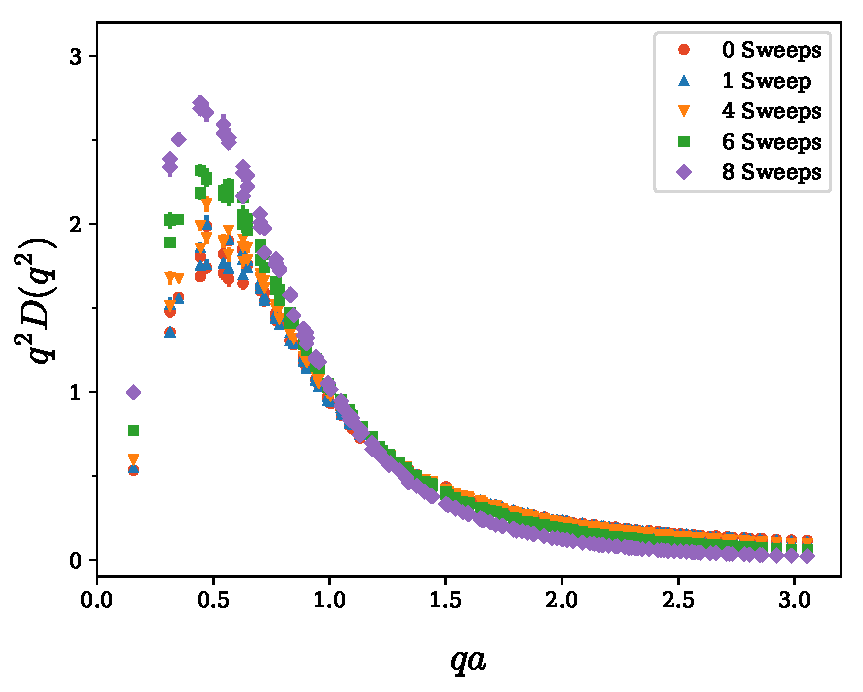
\includegraphics[width=\linewidth]{./ScalarGluComp_q2_1to10sweepsVO.pdf}
\caption[The vortex only propagator after different sweeps of cooling.]{\label{fig:1to10VO}The vortex only propagator after different sweeps of cooling. A trend similar to Fig.~\ref{fig:1to10SweepsCooling} is observed, with enhancement in the infrared and suppression in the UV region.}
\end{figure}
%
We observe that the vortex only and untouched propagators in Fig.~\ref{fig:10SweepsCooling} resemble the gluon propagator under a differing number of sweeps of cooling, as shown in Fig.~\ref{fig:1to10SweepsCooling} and Fig.~\ref{fig:1to10VO}. The vortex only propagator has a peak that sits below the untouched propagator, and the untouched propagator is further suppressed in the $qa\approx 1.5$ region. Following the trend in Fig.~\ref{fig:1to10SweepsCooling} and Fig.~\ref{fig:1to10VO}, this indicates that further cooling on the vortex only propagator would align it with the untouched propagator. This follows from an understanding that the vortex-only configurations are initially much rougher than their untouched counterparts~\cite{Trewartha:2015nna}, and should therefore require additional cooling to obtain agreement with the untouched configurations.\\

To measure the roughness of a configuration we consider the average $\mathcal{O}(a^4)$ three-loop improved action of the lattice divided by the single instanton action $S_0=\frac{8\pi^2}{g^2}$ (see Sec.~\ref{sec:Instantons}), denoted $\bar{S}/S_0$. We observe that for $n<20$ cooling sweeps the vortex-only configurations have a significantly higher action than their untouched counterparts after the same number of sweeps of cooling, as illustrated in Fig.~\ref{fig:ActionMatch}. We therefore seek to find the number of sweeps required to best match the action between the vortex-only and untouched configurations. The results of this procedure are shown in Table \ref{tab:ActionMatch}. If we now plot these matched configurations, we obtain the results shown in Fig.~\ref{fig:UVOActionMatch}. Here we have truncated the plot at large $qa$ to better show the agreement in the mid-$qa$ region. By matching the actions as closely as possible with an integer number of cooling sweeps, we see that there is a better agreement between the untouched and vortex-only gluon propagators.\\

%
\begin{figure}[htb!]
\centering
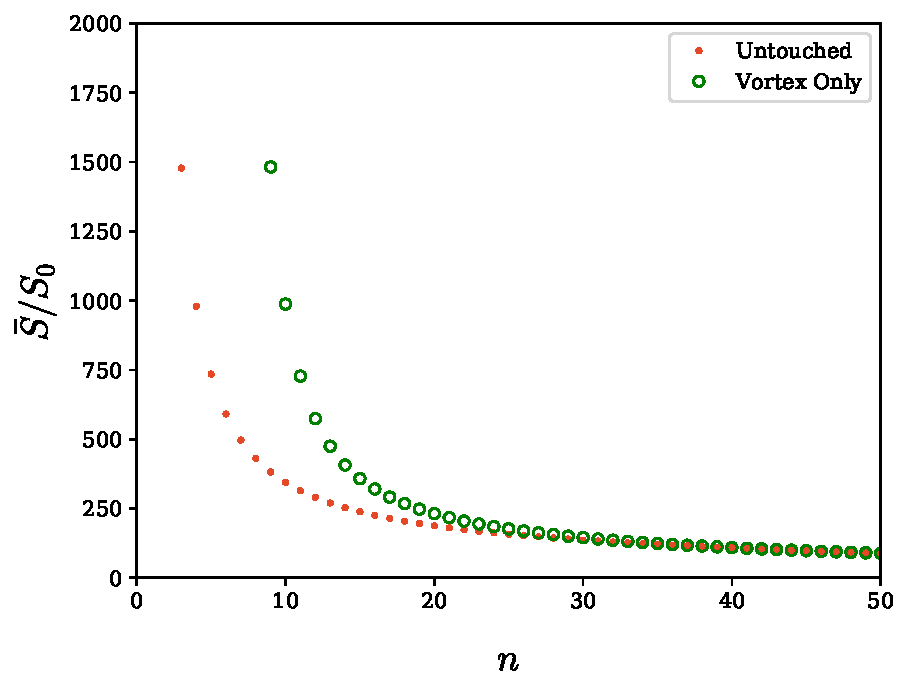
\includegraphics[width=\linewidth]{./ActionMatch.pdf}
\caption[The average action calculated on the untouched and vortex-only configurations as a function of cooling sweeps.]{\label{fig:ActionMatch}The average action calculated on the untouched and vortex-only configurations as a function of cooling sweeps, $n$. The vortex only configurations are initially rougher than the untouched, as evidenced by the higher average action.}
\end{figure}
%
\begin{table}[htb!]
\caption[Comparison of the number of cooling sweeps on the untouched and vortex only configurations required to match the average action.]{\label{tab:ActionMatch}Comparison of the number of cooling sweeps on the untouched ($n_U$) and vortex only ($n_{VO}$) configurations required to match the average action.}
\centering
\begin{tabular}{c | c | c | c}
$n_U$ & $\bar{S}/S_0$ & $n_{VO}$ & $\bar{S}/ S_0$\\
\hline
5 & $734.83$ & 11 & $727.67$\\
10 & $344.22$ & 15 & $357.68$\\
15 & $238.21$ & 20 & $231.19$\\
20 & $187.55$ & 24 & $184.68$\\
25 & $156.92$ & 28 & $155.72$\\
30 & $135.91$ & 32 & $135.61$\\
35 & $120.29$ & 36 & $120.66$\\
40 & $107.08$ & 40 & $109.02$\\
\end{tabular}
\end{table}
%
\begin{figure}[htb!]
\centering
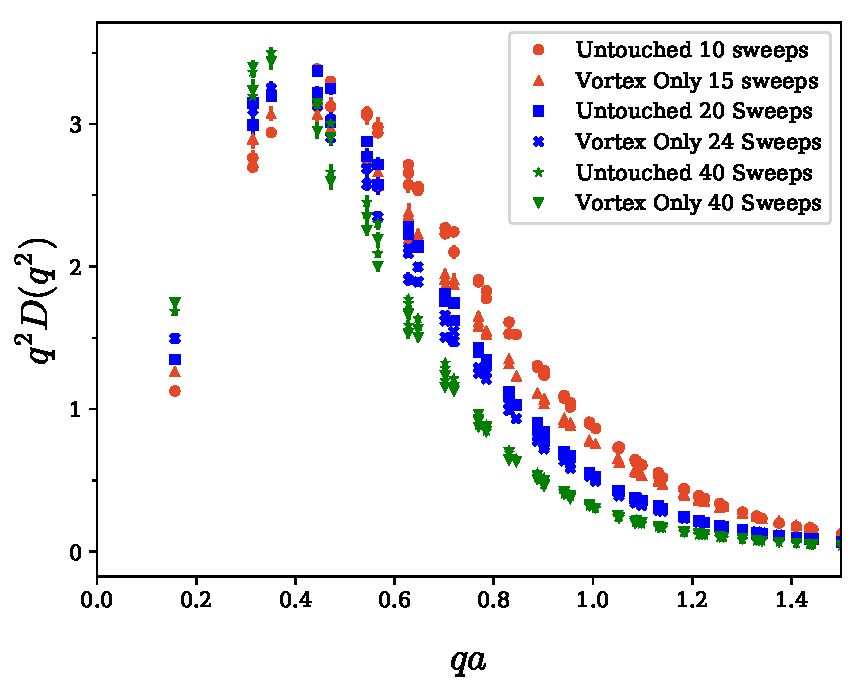
\includegraphics[width=\linewidth]{./ScalarGluComp_q2_UVOActionMatch.pdf}
\caption[Comparison of the gluon propagator on the untouched and vortex only configurations after tuning the number of cooling sweeps to best match the average plaquette action.]{\label{fig:UVOActionMatch}Comparison of the gluon propagator on the untouched and vortex only configurations after tuning the number of cooling sweeps to best match the average plaquette action. This procedure gives a much better agreement in the shape of the gluon propagator from the two configurations.}
\end{figure}
%

\section{Summary}
The results presented above concur with the now significant body of evidence that centre vortices contain the essential degrees of freedom of the Yang-Mills vacuum, such that the application of smoothing enables the recreation of the major features of QCD~\cite{Bertle:2001xd,Trewartha:2015ida,Trewartha:2015nna,Trewartha:2017ive,DelDebbio:1998luz}. We have shown that vortex identification partitions the gluon propagator into low and high momentum modes, with the vortex only configurations encapsulating the majority of the infrared strength. Cross-correlation between the vortex only and vortex removed propagators can be seen to vanish in the ensemble average. By cooling the configurations, we observe that the vortex only configurations are continuously suppressed, while the infrared peak in the untouched and vortex only propagator acquires better agreement. By tuning the number of cooling sweeps to best match the average action of the vortex only and untouched configurations, we can effectively match the gluon propagators obtained from each of these configurations.\\

%
\begin{figure}
\begin{subfigure}[]{0.5\textwidth}
\label{UTcool10}
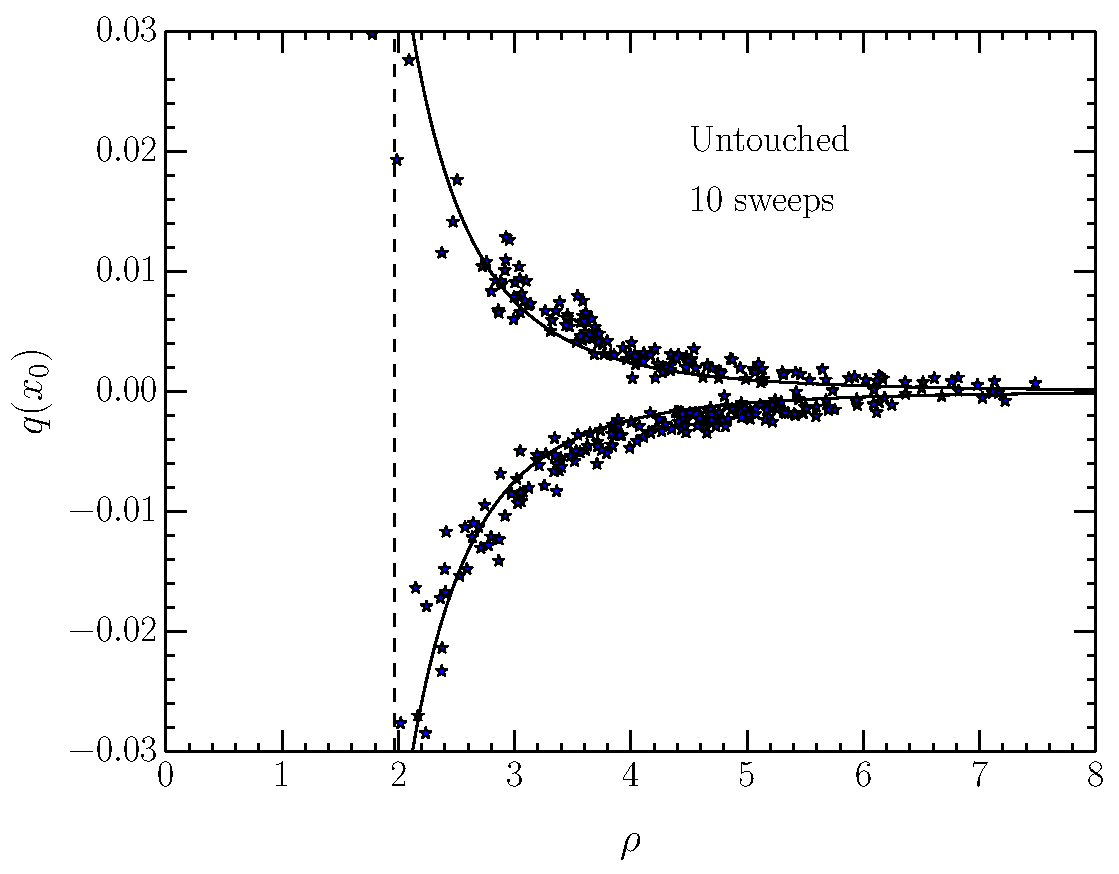
\includegraphics[width=\columnwidth]{./UTcool10.pdf}
\end{subfigure}
\begin{subfigure}[]{0.5\textwidth}
\label{UTcool40}
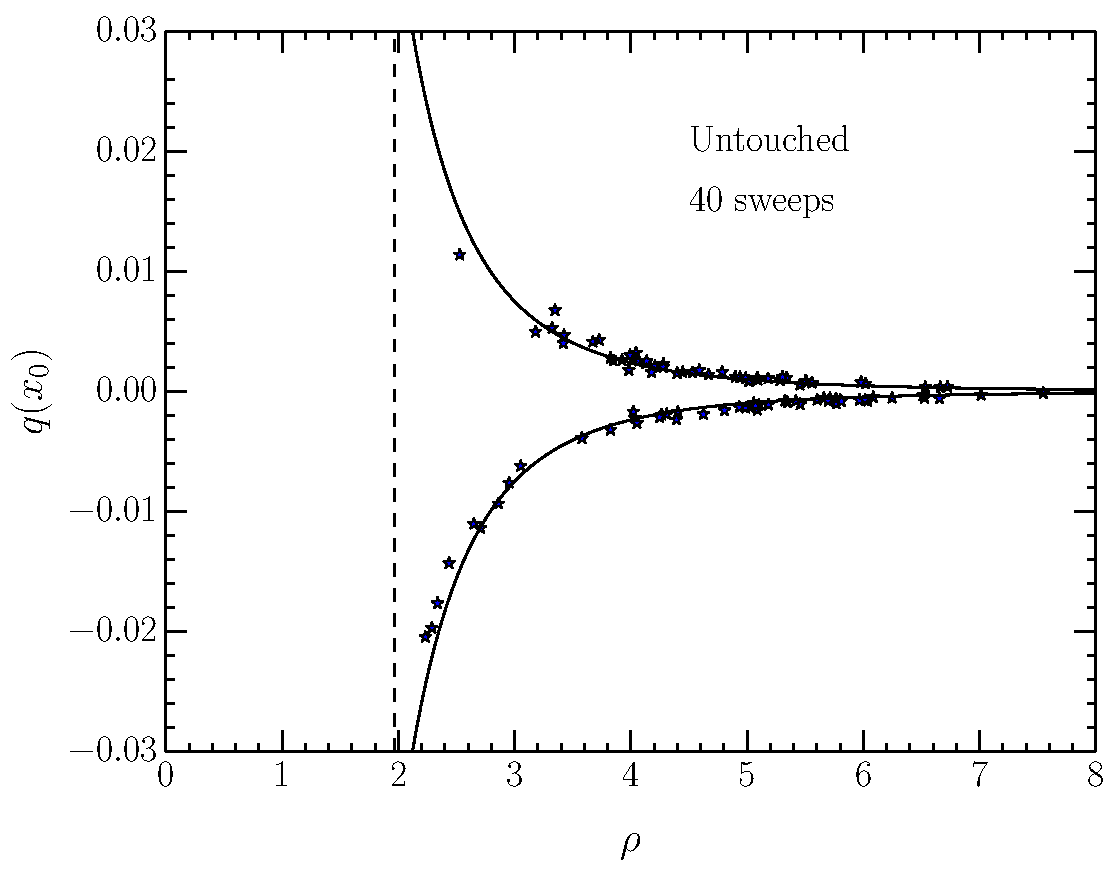
\includegraphics[width=\columnwidth]{./UTcool40.pdf}
\end{subfigure}
\begin{subfigure}[]{0.5\textwidth}
\label{VOcool10}
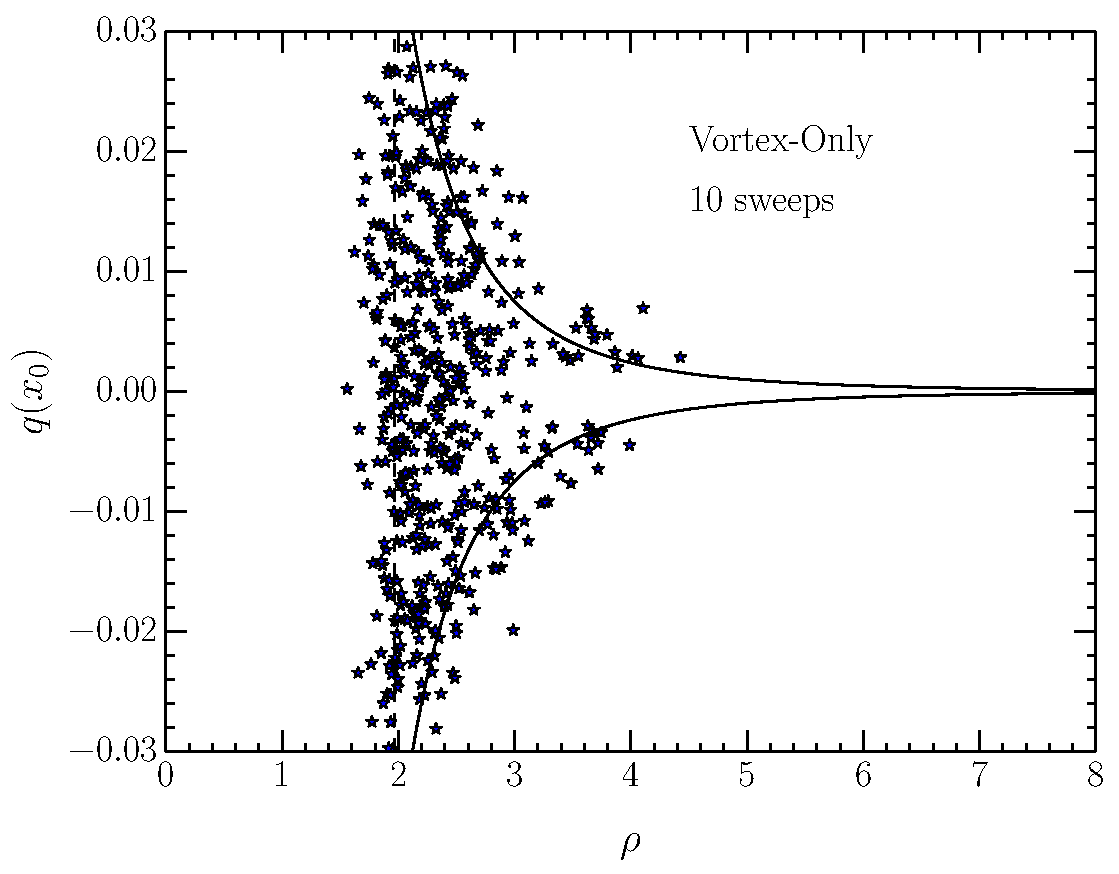
\includegraphics[width=\columnwidth]{./VOPGcool10.pdf}
\end{subfigure}
\begin{subfigure}[]{0.5\textwidth}
\label{VOcool40}
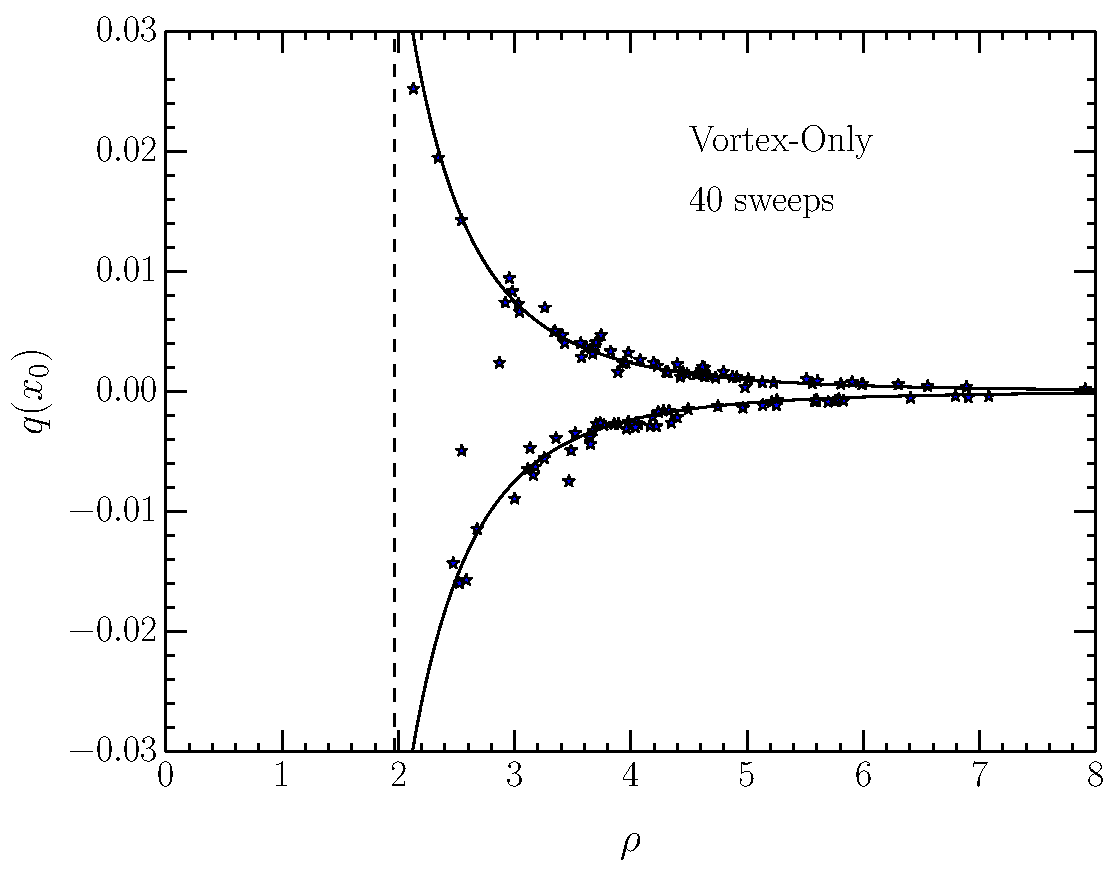
\includegraphics[width=\columnwidth]{./VOPGcool40.pdf}
\end{subfigure}
\begin{subfigure}[]{0.5\textwidth}
\label{VRcool10}
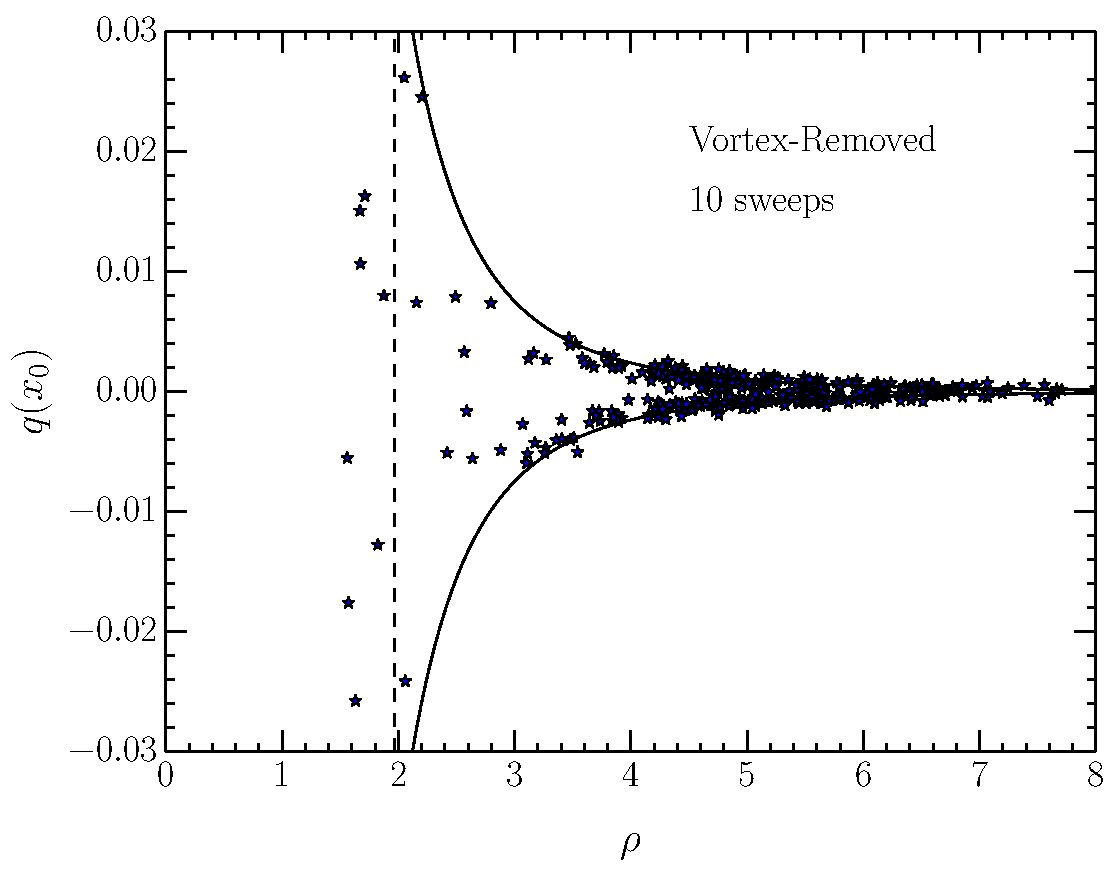
\includegraphics[width=\columnwidth]{./VRcool10.pdf}
\end{subfigure}
\begin{subfigure}[]{0.5\textwidth}
\label{VRcool40}
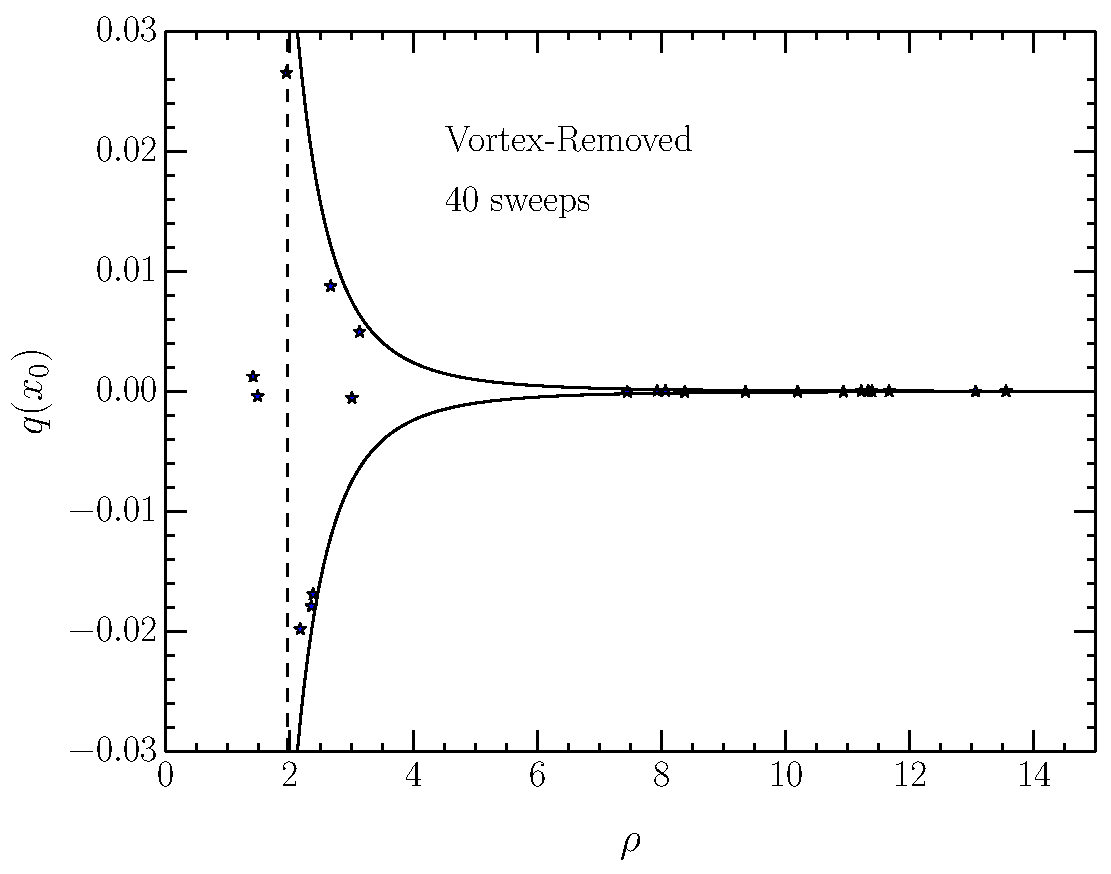
\includegraphics[width=\columnwidth]{./VRcool40.pdf}
\end{subfigure}
\caption[The topological charge at the instanton centre is plotted against the instanton radius for the vortex modified configurations under 10 and 40 sweeps of cooling.]{\label{fig:InstantonRadius} These plots are reproduced from \citet{Trewartha:2015ida}. The topological charge at the instanton centre, $q(x_0)$, is plotted against the instanton radius $\rho$ for the vortex modified configurations under 10 and 40 sweeps of cooling. The solid line represents the theoretical distribution. }
\end{figure}
%
Noting that sufficient smoothing of a vortex-only field generates a topological background of instanton-like objects, we can regard the thin centre vortices as the seeds of instantons. The smoothing process that is applied on the vortex-only configurations raises a question regarding the precise role of vortices in the restoration of the infrared propagator: is it simply the presence of (sufficiently smoothed) vortices or is it more indirectly the reformation of the instanton background? If we examine Fig.~\ref{fig:10SweepsCooling}, we see that after the application of 10 sweeps of cooling the vortex-only propagator has the appropriate qualitative infrared behaviour. Comparing with previous work, in particular Fig.~7 within Ref.~\cite{Trewartha:2015ida} (replicated in Fig.~\ref{fig:InstantonRadius}) which shows the typical distribution of the instanton radius against the topological charge at the centre, we can see that after only 10 sweeps of cooling the vortex-only distribution still deviates significantly from the ideal theoretical instanton relationship. This suggests that it is the smoothed centre vortices that are directly responsible for the infrared structure of the gluon propagator.